\documentclass[border=10pt]{standalone}
\usepackage[T1]{fontenc}
\usepackage{tikz}
\usepackage{amsmath}

\definecolor{garnet}{HTML}{73000A}
\definecolor{atlantic}{HTML}{466A9F}
\definecolor{congaree}{HTML}{1F414D}
\definecolor{warmgrey}{HTML}{676156}
\definecolor{horseshoe}{HTML}{65780B}
\definecolor{rose}{HTML}{CC2E40}
\definecolor{honeycomb}{HTML}{A49137}
\definecolor{bk70}{HTML}{5C5C5C}
\definecolor{bk30}{HTML}{C7C7C7}

\begin{document}
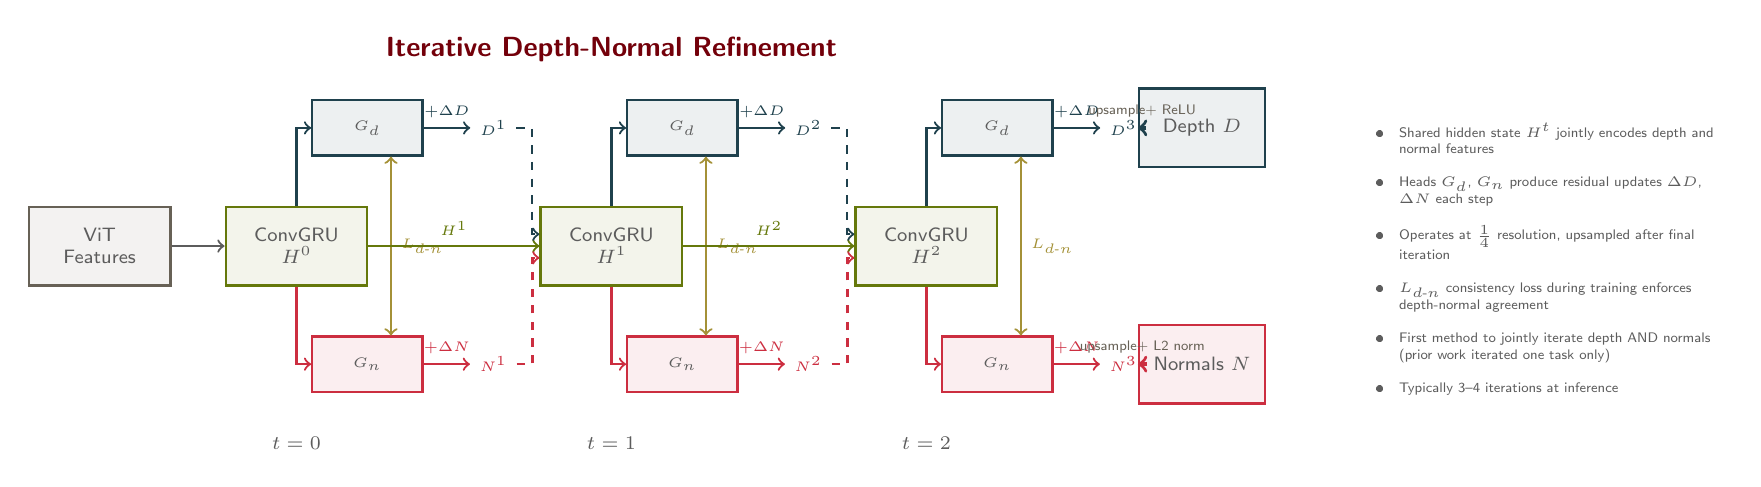
\begin{tikzpicture}[
    block/.style={
        draw=#1, thick, fill=#1!8,
        minimum height=1.0cm, minimum width=1.8cm,
        font=\sffamily\scriptsize, text=bk70, align=center,
    },
    smallblock/.style={
        draw=#1, thick, fill=#1!8,
        minimum height=0.7cm, minimum width=1.4cm,
        font=\sffamily\tiny, text=bk70, align=center,
    },
    arr/.style={->, thick, color=bk70},
    darr/.style={->, thick, color=#1},
    lbl/.style={font=\sffamily\tiny, text=warmgrey},
]

% ════════════════════════════════════════
% Title
% ════════════════════════════════════════
\node[font=\sffamily\bfseries, text=garnet] at (6.5, 6.5) {Iterative Depth-Normal Refinement};

% ════════════════════════════════════════
% Input features
% ════════════════════════════════════════
\node[block=warmgrey] (feats) at (0, 4) {ViT\\Features};

% ════════════════════════════════════════
% ITERATION BOXES (t=0, t=1, t=2)
% Show 3 iterations unrolled left to right
% ════════════════════════════════════════

\foreach \t [count=\i from 0] in {0,1,2} {
    \pgfmathsetmacro{\xbase}{2.5 + \i * 4.0}

    % Hidden state
    \node[block=horseshoe] (gru\t) at (\xbase, 4) {ConvGRU\\$H^{\t}$};

    % Depth head
    \node[smallblock=congaree] (dhead\t) at (\xbase + 0.9, 5.5) {$G_d$};

    % Normal head
    \node[smallblock=rose] (nhead\t) at (\xbase + 0.9, 2.5) {$G_n$};

    % Depth output
    \node[font=\sffamily\tiny, text=congaree] (dout\t) at (\xbase + 2.5, 5.5) {$D^{\the\numexpr\t+1}$};

    % Normal output
    \node[font=\sffamily\tiny, text=rose] (nout\t) at (\xbase + 2.5, 2.5) {$N^{\the\numexpr\t+1}$};

    % GRU → heads
    \draw[darr=congaree] (gru\t.north) |- (dhead\t.west);
    \draw[darr=rose] (gru\t.south) |- (nhead\t.west);

    % Heads → outputs (with + residual)
    \draw[darr=congaree] (dhead\t.east) -- (dout\t.west)
        node[midway, above, font=\sffamily\tiny, text=congaree] {$+\Delta D$};
    \draw[darr=rose] (nhead\t.east) -- (nout\t.west)
        node[midway, above, font=\sffamily\tiny, text=rose] {$+\Delta N$};

    % Consistency loss between depth and normal
    \draw[<->, thick, honeycomb] ([xshift=0.3cm]dhead\t.south) -- ([xshift=0.3cm]nhead\t.north)
        node[midway, right, font=\sffamily\tiny\bfseries, text=honeycomb] {$L_{d\text{-}n}$};
}

% ════════════════════════════════════════
% Connect iterations: features → GRU0
% ════════════════════════════════════════
\draw[arr] (feats.east) -- (gru0.west);

% GRU0 → GRU1 (hidden state carries forward)
\draw[arr, horseshoe] (gru0.east) -- (gru1.west)
    node[midway, above, font=\sffamily\tiny, text=horseshoe] {$H^1$};

% GRU1 → GRU2
\draw[arr, horseshoe] (gru1.east) -- (gru2.west)
    node[midway, above, font=\sffamily\tiny, text=horseshoe] {$H^2$};

% ════════════════════════════════════════
% Feed depth/normal back into next GRU
% ════════════════════════════════════════
% D1 feeds back to GRU1
\draw[darr=congaree, dashed] (dout0.east) -- ++(0.2,0) |- ([yshift=0.15cm]gru1.west);
\draw[darr=rose, dashed] (nout0.east) -- ++(0.2,0) |- ([yshift=-0.15cm]gru1.west);

% D2 feeds back to GRU2
\draw[darr=congaree, dashed] (dout1.east) -- ++(0.2,0) |- ([yshift=0.15cm]gru2.west);
\draw[darr=rose, dashed] (nout1.east) -- ++(0.2,0) |- ([yshift=-0.15cm]gru2.west);

% ════════════════════════════════════════
% Final output
% ════════════════════════════════════════
\node[block=congaree, minimum width=1.6cm] (dfinal) at (14, 5.5) {Depth $D$};
\node[block=rose, minimum width=1.6cm] (nfinal) at (14, 2.5) {Normals $N$};

\draw[darr=congaree, very thick] (dout2.east) -- (dfinal.west)
    node[midway, above, font=\sffamily\tiny, text=warmgrey] {upsample\\+ ReLU};
\draw[darr=rose, very thick] (nout2.east) -- (nfinal.west)
    node[midway, above, font=\sffamily\tiny, text=warmgrey] {upsample\\+ L2 norm};

% ════════════════════════════════════════
% Iteration labels
% ════════════════════════════════════════
\node[font=\sffamily\scriptsize, text=bk70] at (2.5, 1.5) {$t = 0$};
\node[font=\sffamily\scriptsize, text=bk70] at (6.5, 1.5) {$t = 1$};
\node[font=\sffamily\scriptsize, text=bk70] at (10.5, 1.5) {$t = 2$};

% ════════════════════════════════════════
% Bullet points on the right
% ════════════════════════════════════════
\node[font=\sffamily\tiny, text=bk70, anchor=north west, align=left, text width=5cm]
    at (15.5, 6.0) {%
    \begin{itemize}
    \setlength{\itemsep}{2pt}
    \item Shared hidden state $H^t$ jointly encodes depth and normal features
    \item Heads $G_d$, $G_n$ produce residual updates $\Delta D$, $\Delta N$ each step
    \item Operates at $\tfrac{1}{4}$ resolution, upsampled after final iteration
    \item $L_{d\text{-}n}$ consistency loss during training enforces depth-normal agreement
    \item First method to jointly iterate depth AND normals (prior work iterated one task only)
    \item Typically 3--4 iterations at inference
    \end{itemize}%
    };

\end{tikzpicture}
\end{document}
